\subsection{The Large Hadron Collider}
\begin{frame}{The Large Hadron Collider (LHC)}
\begin{columns}
\column{0.5\textwidth}

\begin{itemize}
    \item \textbf{\textcolor{structurColor}{$pp$ collisions,} up-to $\sqrt{s} = $ 13 TeV}
    %\item Collision rate of $\sim$ 40 MHz (\textbf{\textcolor{HHred}{challenging trigger $\sim$ kHz}})
    \item\textbf{Four large experiments} 
\end{itemize}
\column{0.5\textwidth}
\begin{figure}
        \centering
        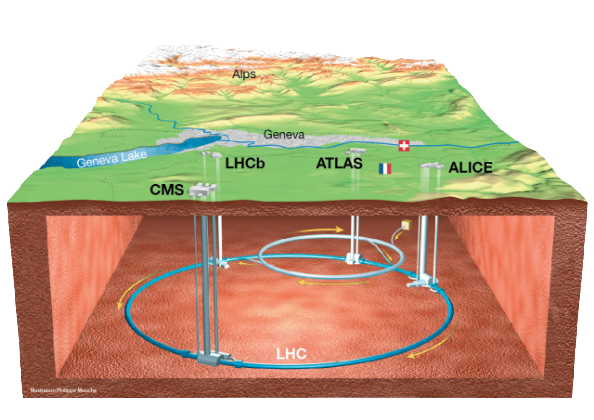
\includegraphics[width=1.1\textwidth]{Part2/Img/b_RTU_a_schematic_depiction_of_the_lhc-removebg-preview.png}
\end{figure}    
\end{columns}

\end{frame}

\subsection{The ATLAS detector}
\begin{frame}{The ATLAS detector}

\begin{columns}
\column{0.65\textwidth}
\begin{figure}
    \centering
    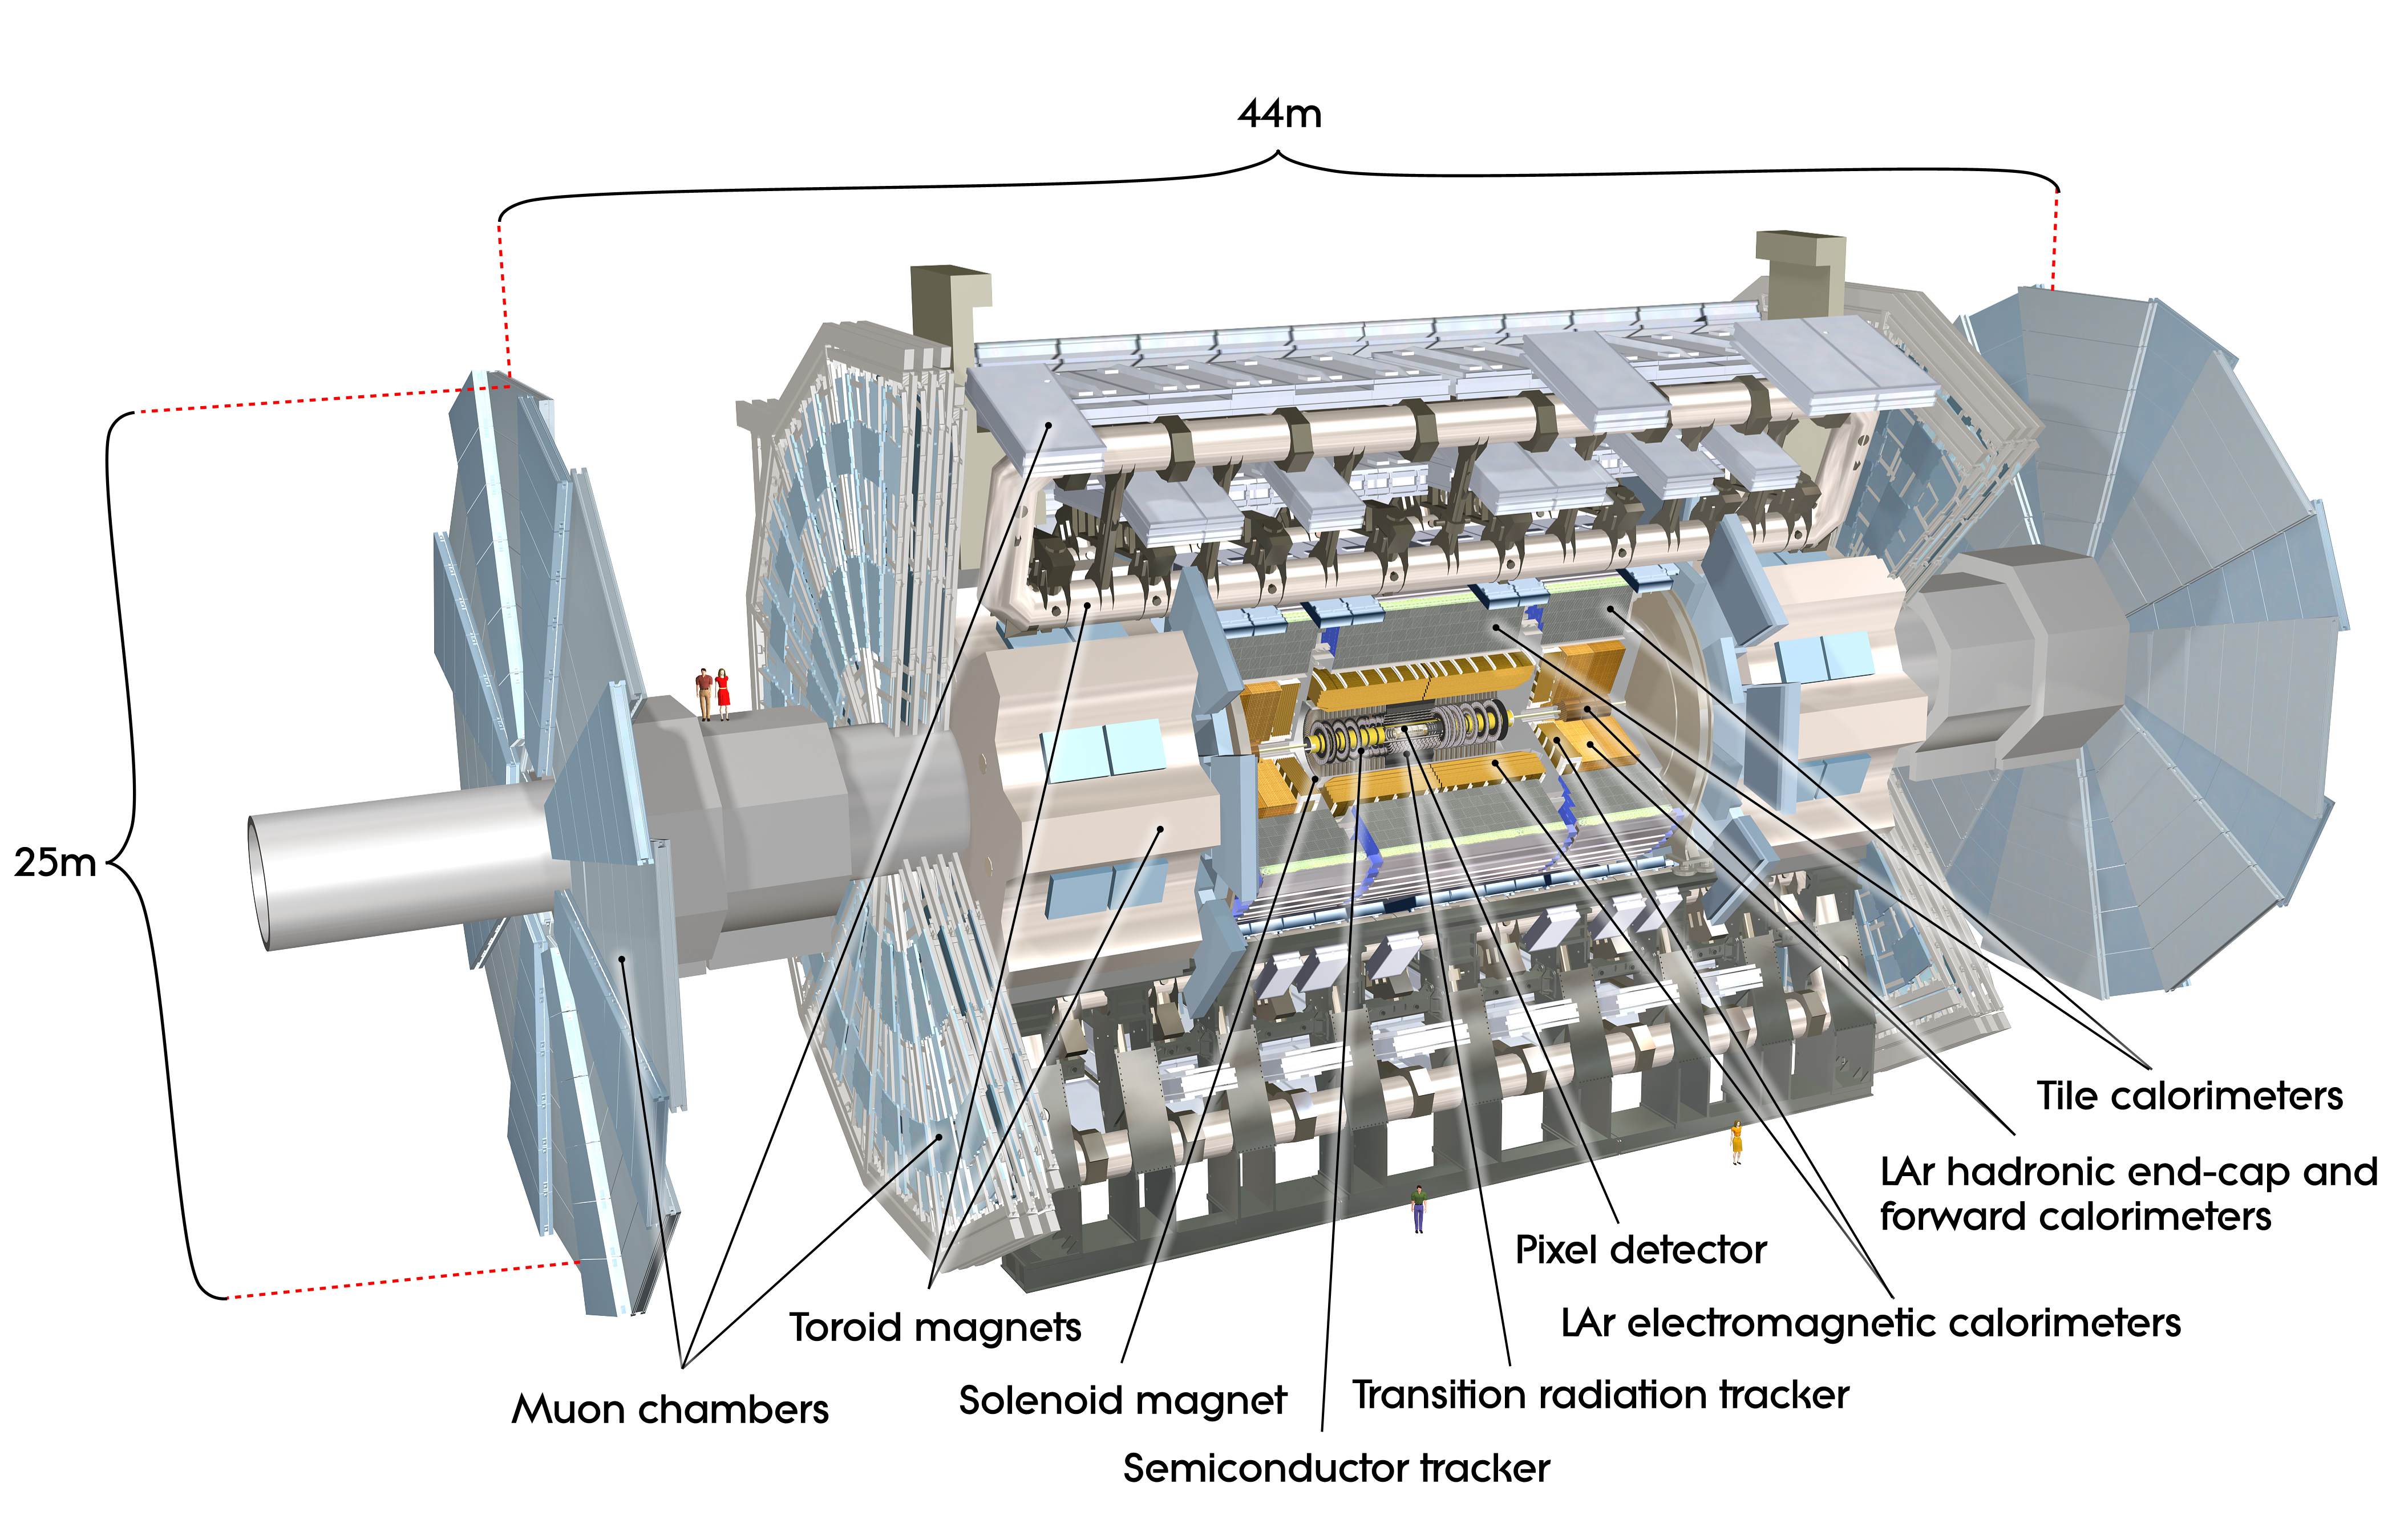
\includegraphics[width=1.\textwidth]{Part2/Img/ATLAS_sketch.jpg}
\end{figure}

\column{0.35\textwidth}

\begin{itemize}
    \item \textbf{Different sub-detectors}
    \item \textbf{Cylindrical} coordinate system
\end{itemize}
\begin{figure}
    \centering
    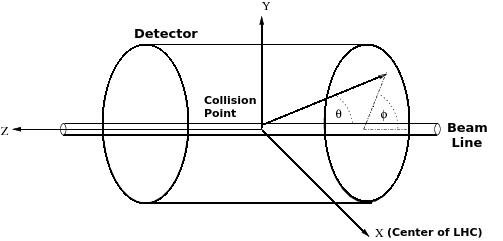
\includegraphics[width=1.\textwidth]{Part2/Img/ATLAS_Sys.jpeg}
\end{figure}
\begin{equation*}
    (p_T, \phi, \eta)
\end{equation*}
\begin{equation*}
    \textcolor{HHblue}{\eta = -\ln[\tan\frac{\theta}{2}]}
\end{equation*}
\end{columns}

\end{frame}

%\subsection{Particles reconstruction}
%\begin{frame}{Particles reconstruction}

%\begin{columns}
%\column{0.4\textwidth}

%\begin{itemize}
%    \item \textcolor{HHred}{Electrons} \& \textcolor{HHred}{Photons}
%    \begin{itemize}
%        \item EM cluster (+ ID track)
%    \end{itemize}
%    \item \textcolor{cadmiumorange}{Muons}
%    \begin{itemize}
%        \item Tracks
%    \end{itemize}
%    \item \textcolor{applegreen}{Hadrons} (jets)
%    \begin{itemize}
%        \item EM/Had clusters (+ ID track)
%    \end{itemize}
%    \item \textcolor{HHturquoise_l}{Neutrinos}
%    \begin{itemize}
%        \item Missing momentum
%    \end{itemize}
%\end{itemize}
%\column{0.6\textwidth}
%\begin{figure}
%    \centering
%    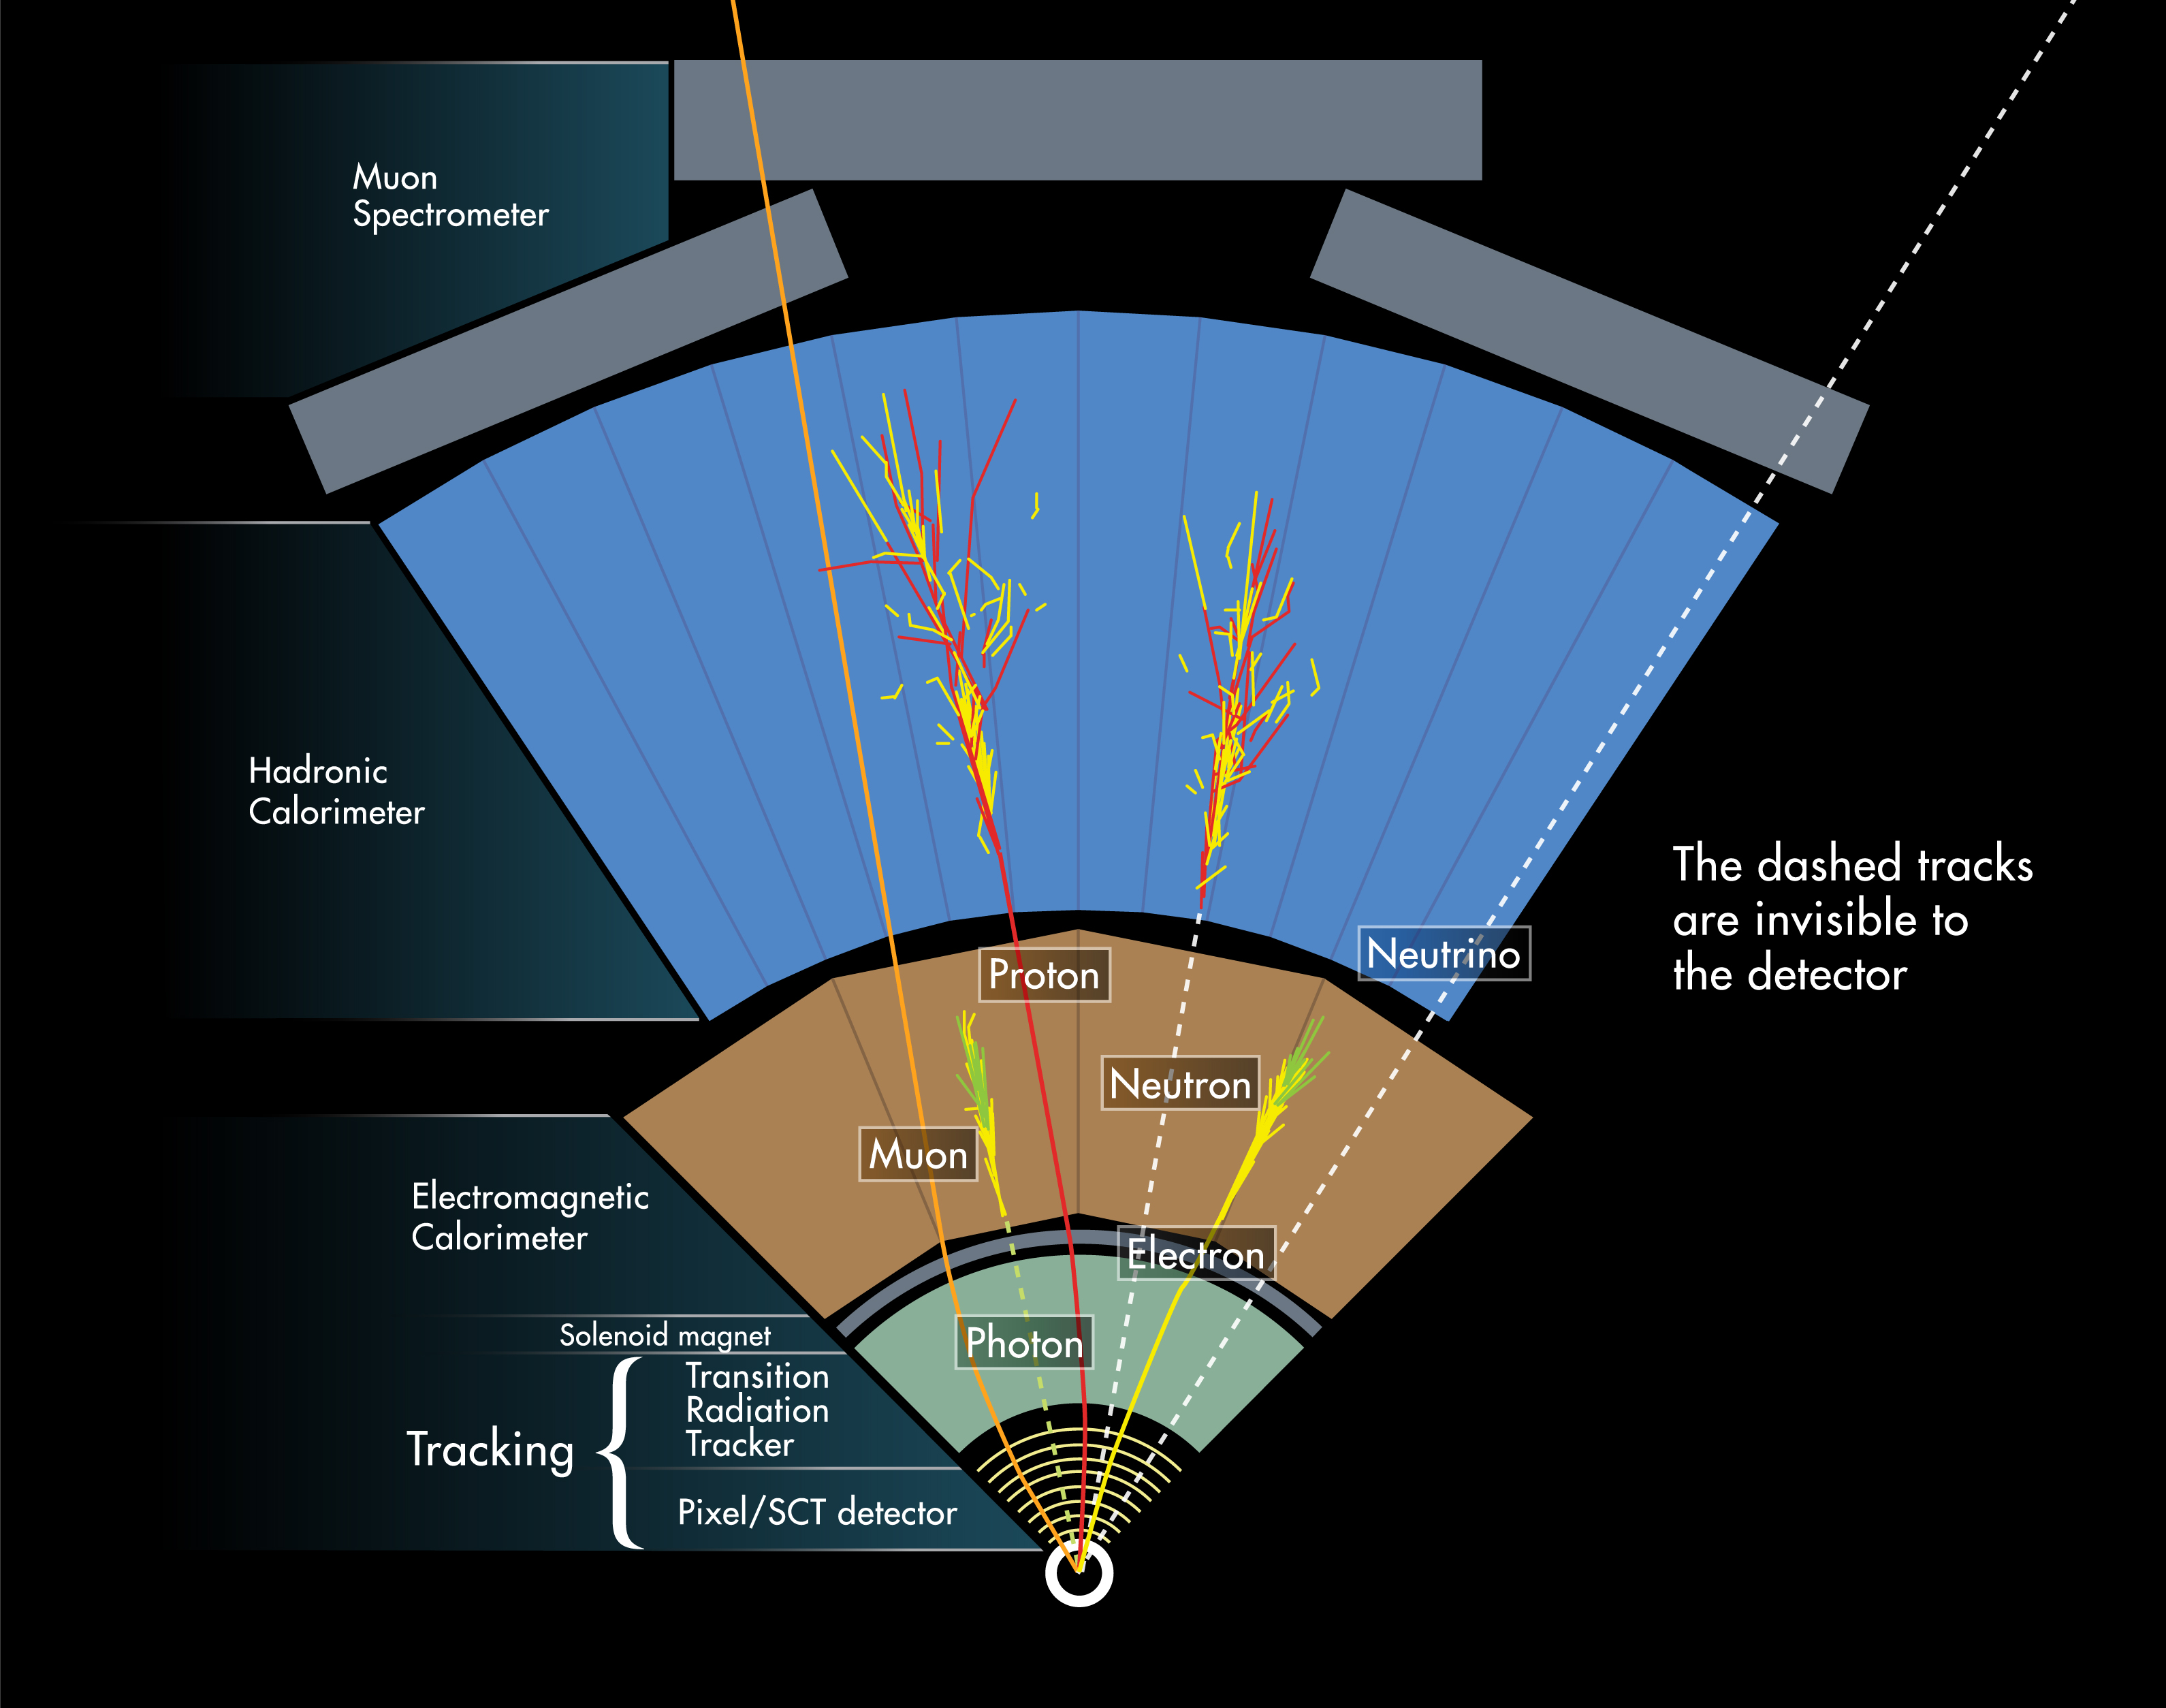
\includegraphics[width=1.\textwidth]{Part2/Img/Particle_detection.jpg}
   
%\end{figure}

%\end{columns}

%\end{frame}
\begin{frame}{Run-2 data taking}
    
\begin{textblock*}{5cm}(14.1cm, 3.2cm) % {block width} (coords) 
   \rotatebox{90}{\textbf{\textcolor{HHred}{--------------------------}}}
\end{textblock*}
\begin{textblock*}{5cm}(13.8cm, 4.1cm) % {block width} (coords) 
   \rotatebox{90}{\textbf{\textcolor{HHred}{Thesis begins}}}
\end{textblock*}
\begin{columns}
\column{0.5\textwidth}
\begin{itemize}
    \item Run-2 period: 2015-2018
    \item Integrated luminosity used for presented analysis: \textbf{139 fb$^{-1}$}
\end{itemize}


%\textcolor{HHblue}{\underline{Pile-up}}:
%\begin{itemize}
%    \item Dense environments 
%    \item \textbf{challenge!}
%\end{itemize}

%\begin{figure}
%    \centering
%     \fcolorbox{HHblue}{HHwhite2}{
%    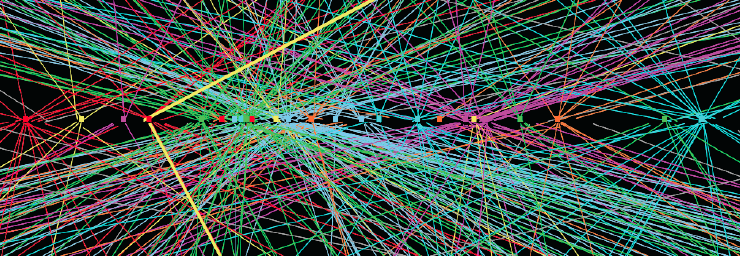
\includegraphics[width=0.8\textwidth]{Part2/Img/PileupEvent.png}
%    }
%\end{figure}
\column{0.5\textwidth}

\begin{textblock*}{5cm}(10cm, 5.4cm) % {block width} (coords) 
  \textcolor{black}{2015-2016 \\ (36 fb$^{-1}$)}
\end{textblock*}

\begin{figure}
    \centering
     \fcolorbox{HHred}{HHwhite2}{
    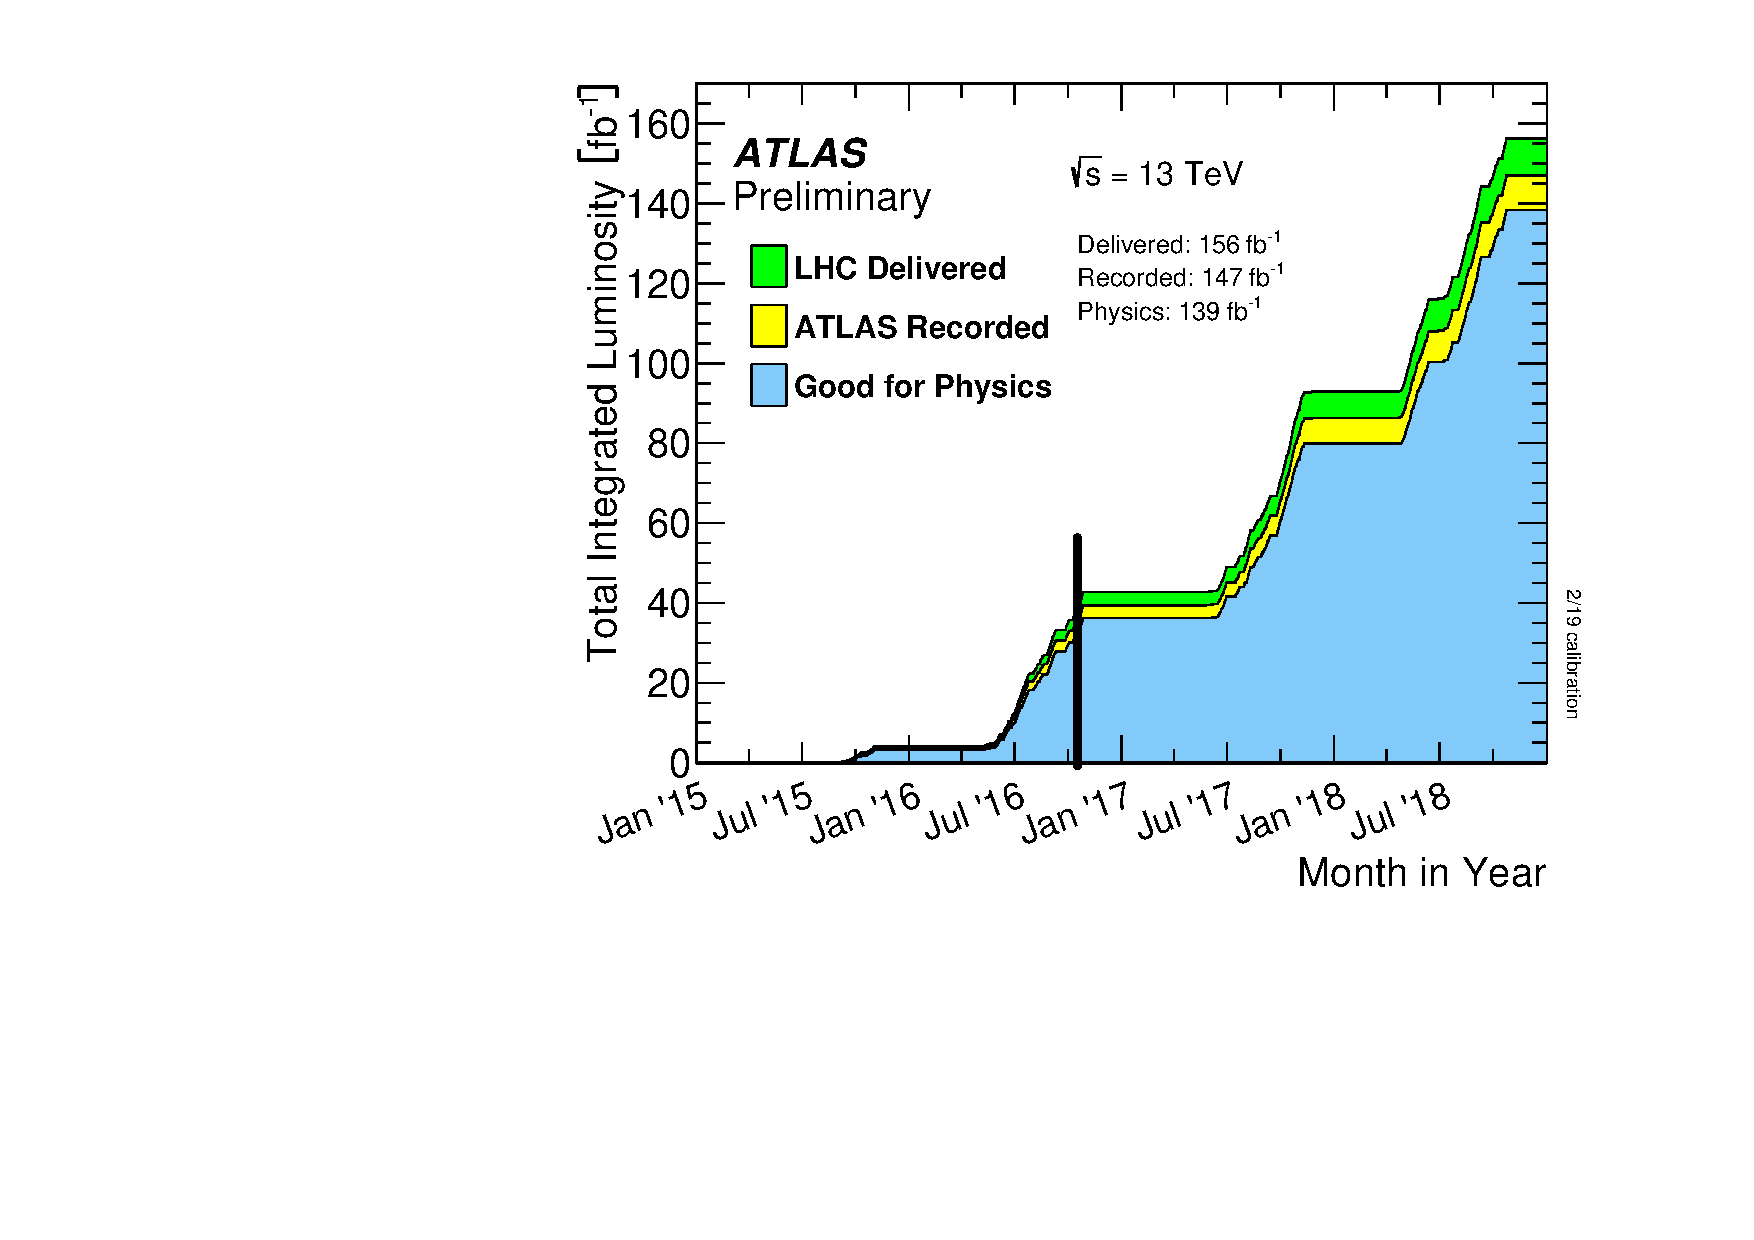
\includegraphics[width=1.\textwidth]{Part2/Img/intlumivstimeRun2DQall_edit.pdf}
    }
\end{figure}

%\begin{figure}
%    \centering
%     \fcolorbox{HHblue}{HHwhite2}{
%    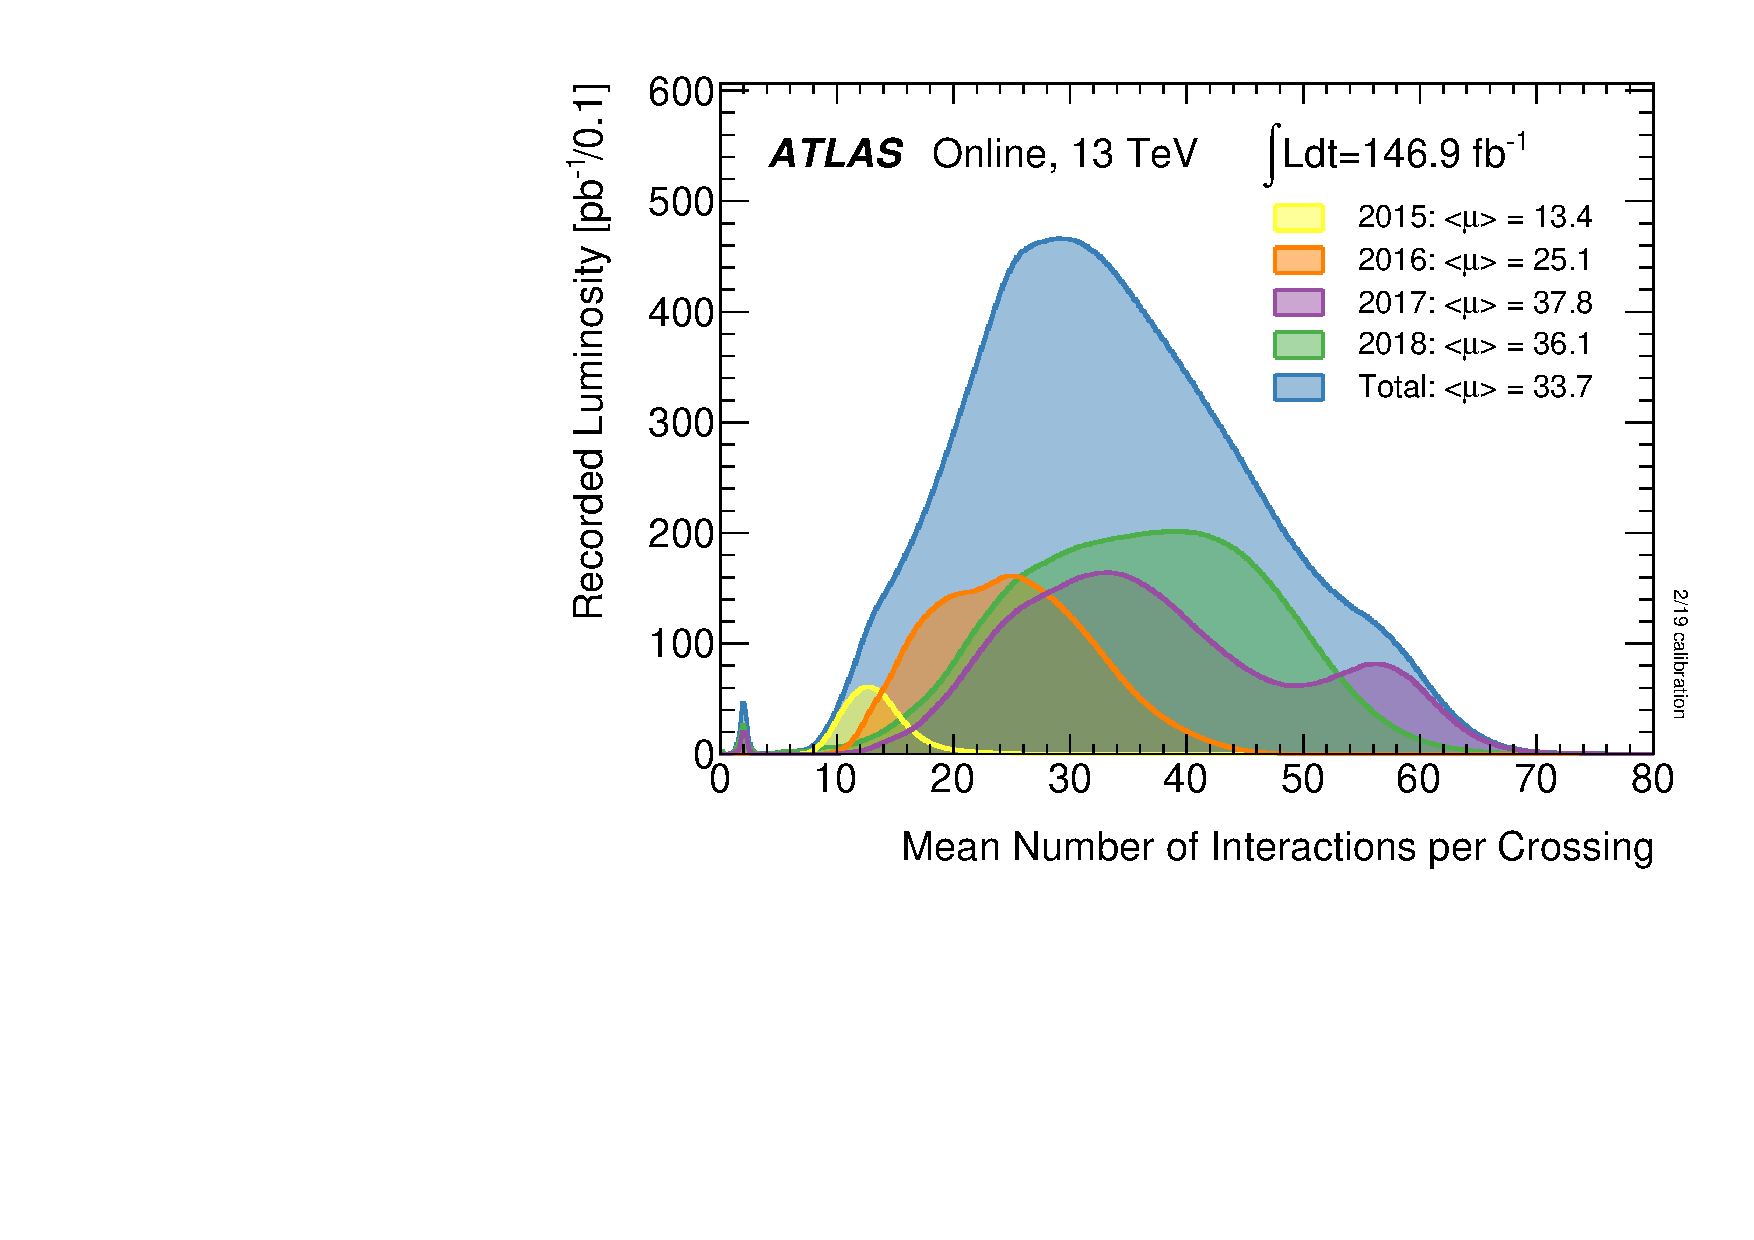
\includegraphics[width=0.55\textwidth]{Part2/Img/mu_2015_2018.pdf}
%    }
%\end{figure}

\end{columns}  
\end{frame}

\begin{frame}{Where are we with HH$\to b\bar{b}\gamma\gamma$?}
 
\begin{textblock*}{5cm}(8.5cm,2.8cm) % {block width} (coords) 
   \textcolor{applegreen}{\textbf{\href{https://link.springer.com/article/10.1007\%2FJHEP11\%282018\%29040}{JHEP 11 (2018) 040}}}
\end{textblock*}

\begin{itemize}
    \item Previous analysis: \textbf{\textcolor{applegreen}{2015-2016 data (36 fb$^{-1}$)}}
    \begin{itemize}
        \item $\frac{\sigma_{ggF}}{\sigma^{SM}}(HH)$ limit: \textbf{\textcolor{structurColor}{22}} (Exp. \textbf{28}) at 95\% CL
        \item $\kappa_{\lambda}$ constrain: \textbf{\textcolor{structurColor}{[-8.2, 13.2]}} (Exp. \textbf{[-8.3, 13.2]})
    \end{itemize}
\pause    
    \item My thesis: \textbf{\textcolor{HHred}{Full run-2 data (139 fb$^{-1}$)}}
    \begin{itemize}
        \item Improve the analysis sensitivity with different tools
    \end{itemize}
\end{itemize}    
\vspace{1em}
\begin{tabular}{lccc}
    \hline 
    \hline
     & HH & HH$\to b\bar{b}\gamma\gamma$ & $\sim$10\% eff. \\
     \hline
    Events  & 4.3k & 11 & $\mathcal{O}(1)$ \\
      \hline\hline 
\end{tabular}    
\end{frame}